%!TEX root = ../main.tex

\chapter{The \gerda\ experiment}\label{chap:gerda}

The GERmanium Detector Array (\gerda) experiment has been proposed in
2004~\cite{gerda-proposal} to search for neutrinoless double-beta decay with High-Purity
Germanium detectors (HPGe) enriched in the \gesix\ double-beta emitter. The proposal lies
in the path opened by the Heidelberg-Moscow (\hdm)~\cite{Klapdor2001} and
\igex~\cite{Aalseth2002} experiments, aiming to develop the germanium technology towards
large-scale, background-free experimental conditions that could tackle the scale of
$\mathcal{O}(10^{26})$~yr sensitivity on the neutrinoless double-beta decay half-life. The
history of the achievements in \thalfzero\ limit setting and background level with \gesix\
is presented in \cref{img:exp:ge76-history}, top. On the bottom plot, a zoom in the
\gerda\ data taking period showing the experimental progresses in terms of \thalfzero\
sensitivity, lower limit and collected active exposure.  \gerda\ data taking officially
ended in November 2019 after hitting the target total background-free exposure of 100~\kgyr\ and
establishing itself as the leading experiment in the field in terms of lowest background
level ever achieved around \qbb~\cite{Agostini2019a}.

\blocktitle{\gerda\ \\ phases}
Since the start of the data taking in 2008 the experiment, located in hall~A of the
Laboratori Nazionali del Gran Sasso (LNGS) in Italy, has been running through two distinct
experimental phases (\phaseone\ and \phasetwo). Detectors from the former \hdm\ and \igex\
experiments (of semi-coaxial geometry) along with newly produced diodes (of \bege\
geometry type, shorthand for Broad Energy Germanium detectors) were deployed bare into
liquid argon (LAr) during \phaseone, following a suggestion by ref.~\cite{Heusser1995},
for a total amount of 21.3~kg of germanium. \phaseone\ ended in June 2013 with a total
exposure of 21.6~\kgyr\ and a background index in the region of interest of
\pIbi~\cite{Agostini2016}.  Shortly after that the upgrade works for \gerda\ \phasetwo\ started:
a new event veto system based on the LAr scintillation light was installed along with an
additional 20~kg of \bege-type detectors.  The newly designed veto system set the stage for a
significant reduction of the background index (BI) down to the \powctsper{-4} scale, allowing
\gerda\ to seamlessly run in background-free conditions for its full second experimental phase
and surpass the \powtenyr{26} sensitivity threshold in April 2018~\cite{Agostini2019a}.
Data taking was then stopped again to permit a third hardware upgrade, during which
another 9.6~kg of enriched germanium in the form of five inverted-coaxial geometry
detectors was deployed\footnote{Note however that a semi-coaxial detector (\ANG{1}) and
the natural \GTF{} detectors were removed.}. Moreover, the LAr veto system was exchanged
with a more efficient one, thanks to the denser fiber curtain and the addition of a shroud
enclosing the central string, now consisting of inverted-coaxial detectors only. This last
part of \phasetwo, which will be referred as \phasetwop\ in the following, ended in
November 2019 after collecting the total exposure of \gexpo and
establishing the final \gerda\ upper limit on the neutrinoless double-beta decay half-life
of \gerdafinallimit. When generally referring to the \phasetwo\ period, if not specified
in the following, \phasetwop\ must be considered as implicitly included.
\begin{figure}
  \centering
  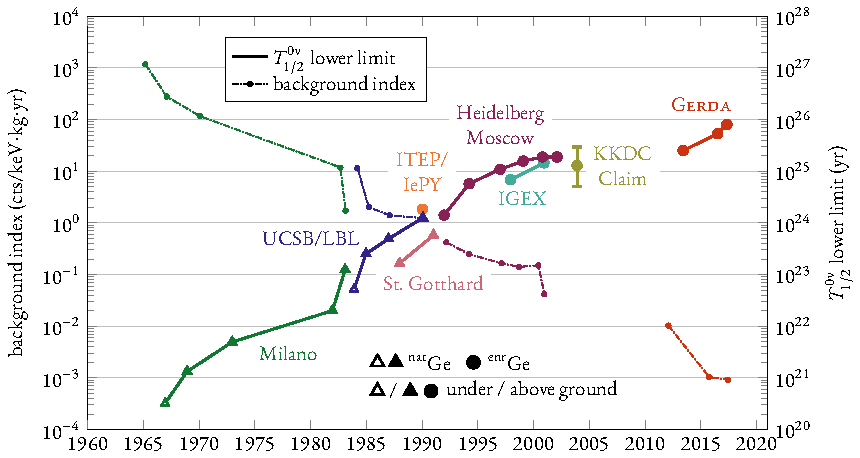
\includegraphics{plots/history/0nbb-ge76-history.pdf}
  \caption[placeholder]{%
    History of neutrinoless double-beta decay experiments with \gesix. Each point
    correspond to a specific journal publication. Top panel: evolution of \thalfzero\
    lower limits and background index in the ROI. Bottom panel: evolution of the
    accumulated exposure and \mbb\ upper limits, if reported in the publication. Note that
    these \mbb\ constrains include the theoretical uncertainty on matrix elements as known
    at the time of publication. Some \hdm\ publications report a single \mbb\ value. 90\%
    C.L.~limits, if available, are preferred to 68\% C.L.~limits. Different markers are
    used in the bottom panel to distinguish between experiments above or under ground,
    experiments using natural or isotopically-enriched germanium\protect\footnotemark.
  }\label{img:exp:ge76-history}
\end{figure}
\footnotetext{Data collected for the history plots can be downloaded in JSON format at
\url{https://github.com/gipert/phd-thesis/src/img/plots/history/data/ge76-history.json}.}
\begin{figure}
  \centering
  \includegraphics{plots/history/gerda-history-vs-exposure.pdf}
  \caption{%
    Evolution of sensitivity and \thalfzero\ limits set by \gerda\ over accumulated
    exposure. The almost perfect linear increase of the sensitivity for limit setting
    demonstrates the background-free conditions in which the experiment has been operating
    in its second phase. Deviations of the observed limit from the expectations for no
    signal are due to the particular statistical realization.
  }\label{img:exp:gerda-history}
\end{figure}
\newpar
The \phasetwop\ upgrade is partly also a test bench for the next-generation successor of
\gerda\ in the field of double-beta decay physics with \gesix, the LEGEND experiment. The
collaboration, formed in October 2016 from the \gerda\ and \majorana~\cite{Abgrall2014}
(the latter experiment is searching for \onbb\ with germanium detectors at the Sanford
Underground Research Facility (SURF) in USA), pursues the goal of building a tonne-scale
\gesix\ experiment and reaching the $\mathcal{O}(10^{28})$~yr sensitivity scale. The first
phase of the experiment, LEGEND-200, will deploy 200~kg of germanium in the existing \gerda\
infrastructure at LNGS and it is currently in commissioning phase.
\newpar
As the present thesis work focuses on \gerda\ \phasetwo\ data, the description of the
experimental setup and the main analysis techniques given in the following will be limited
to that time period. The chapter is structured as follows. In \cref{sec:gerda:setup} a
general overview of the \gerda\ \phasetwo\ (and \phasetwop) apparatus is given. In
\cref{sec:gerda:cuts} the working principles of the main background reduction techniques
that allow \gerda\ to operate in the background-free regime are outlined. The application
of these event-selection criteria to the \phasetwo\ data, the statistical analysis of the
events at \qbb\ and the final results are presented in \cref{sec:gerda:ana}.

\section{Overview of the \phasetwo\ experimental setup}%
\label{sec:gerda:setup}

The \gerda\ experiment is located in hall~A of the LNGS laboratories, at a depth of about
3500~m water equivalent, to suppress cosmogenically-induced background
sources~\cite{Wiesinger2018}. The germanium detectors are arranged into strings within a
cryostat filled with 64~m$^3$ of liquid argon (LAr), which acts as a shielding and cooling
medium at the same time. The cryostat itself is enclosed by a large tank containing
590~m$^3$ of ultra-pure water.  Besides the additional shielding effect, this water layer
act as a medium for a \v{C}erenkov veto system with 66 photomultiplier tubes (PMTs)
against muons. An array of scintillating panels is installed on the top of the clean room
to complete the muon veto system~\cite{Freund2016} (see \cref{fig:setup:pictures}a). A
simplified representation of the experimental setup is given in \cref{fig:setup:overview},
together with a picture taken from the outside.

\begin{figure}
  \centering
  \includegraphics[width=\textwidth]{setup/gerda-overview.pdf}
  \caption{%
    On the right: artist view of the \gerda\ experimental setup. On the left: a picture of
    taken during the inauguration in November 2010. The experiment, installed in hall A of
    the Laboratori Nazionali del Gran Sasso in Italy, deploys an array of germanium detectors
    enriched in \gesix\ bare in liquid argon, together with a liquid argon scintillation
    light veto system. The cryostat is submerged in a water tank to provide additional
    shielding from external background sources. A plastic scintillating panel system is
    installed on the top of the whole structure as an active muon veto, together with the
    water tank.
  }\label{fig:setup:overview}
\end{figure}

\blocktitle{detectors}
The \gerda\ \phasetwo\ array is organized in 7 vertical strings, holding 40 detectors in
total. The detectors can be divided in three groups: the \bege\ detectors, the
semi-coaxial \m{ANG} and \m{RG}, and the semi-coaxial \m{GTF} detectors. The detectors of
the first two groups are made of germanium enriched in \gesix, the third group includes
detectors with natural isotopic germanium abundance. During the upgrade works for
\phasetwop\ in 2018 four enriched inverted-coaxial \IC{} detectors were introduced to
replace the three \GTF{} detectors in the central string, for a total of 41 detectors
deployed.
\newpar
All \gerda\ HPGe detectors are made of high-purity p-type germanium, which is initially
used to pull crystals, typically fuse-shaped (see for example fig.~4.1a in
\cite{Yonenaga2019}).  Crystals are then cut in slices, and each of them is further
processed to obtain the final detector geometry. The electrodes for signal read-out and
voltage biasing are then fabricated on the detector surface. The \nplus\ contact, where the
external voltage is applied, `wraps around' the detector. It is obtained by deposition of
a lithium layer on the surface, which diffuses below the surface until a depth of
$\sim$1~mm during the subsequent thermal annealing cycles. The presence of lithium
impurities effectively creates a region with decreased charge collection efficiency (CCE),
or `dead-layer', even when biased at full-depletion voltages.  In this region, the CCE is
zero at the surface and reaches its maximal value at the full charge collection depth
(FCCD). The \pplus\ electrode, where the signal is read out, is instead fabricated by boron
implantation, and the dead layer it produces is typically smaller, at the level of
hundreds of microns. The two conductive surfaces are separated by an insulating region,
which is typically produced by excavating a `groove'. In some cases such groove is
passivated by deposition of a germanium-oxide layer.
\newpar
\blocktitle{%
  \includegraphics[width=15mm]{gedet/BEGe.png}\\
  \includegraphics[width=15mm]{gedet/SemiCoax.png}\\
  \vspace{2mm} % tweak
  \includegraphics[width=15mm]{gedet/InvCoax.png}%
}
The \gerda\ \phasetwo\ detectors before the 2018 upgrade can be classified according to
two different geometry types: semi-coaxial and \bege. In the semi-coaxial design, a
bore-hole is excavated along the central axis to accomodate the \pplus\ electrode. With
such a configuration, relatively large detector masses can be achieved, of the order of
2--3~kg. The \ANG{} (5), \RG{} (2) and \GTF{} (3) detectors, inherited from the \hdm\ and
\igex\ experiments and already used in \phaseone, are of the semi-coaxial type. Their
total mass amounts to 23.2~kg of germanium, while the enrichment fractions are in the
85.5--88.3\% range. For \phasetwo, 20~kg of germanium enriched at 87.8\% was procured by
the \gerda\ collaboration for the production of 30 new diodes of the \bege\ type. The
Broad Energy Germanium detector design does not include a bore-hole, therefore the \pplus\
contact is a small, dot-shaped surface at the center of one of the two detector sides. The
absence of a bore-hole makes this kind of detectors harder to fully deplete, requiring
lower impurity concentrations and smaller masses, generally lower than 1~kg. A detailed
description of the characteristics of the \bege\ detectors, from germanium procurement to
diode production can be found in~\cite{Agostini2015e, Agostini2018a, Agostini2019}. For
\phasetwop\ four new enriched \IC{} detectors of the inverted-coaxial type were fabricated
and deployed in place of the natural \GTF{} detectors. This new inverted-coaxial geometry
design includes a dot-shaped \pplus\ contact, to enable the \bege-like pulse-shape
discrimination features, and a bore-hole of the other side, to make it possible to achieve
large detector masses. Details about the production and characterization of the  four
inverted-coaxial detectors deployed in \gerda\ \phasetwop\ can be found
in~\cite{inverted-paper}.

\begin{figure}
  \centering
  \includegraphics[height=7cm]{gedet/phII-array.png}%
  \hspace{0.5cm}%
  \includegraphics[width=4cm, trim=0 -4cm 0 0]{gedet/phII-array-calib.png}%
  \hspace{0.5cm}%
  \includegraphics[height=7cm]{gedet/phIIp-array.png}
  \vspace{1cm}

  \includegraphics[width=0.48\textwidth]{gedet/phII-array-2D.pdf}%
  \hspace{0.04\textwidth}%
  \includegraphics[width=0.48\textwidth]{gedet/phIIp-array-2D.pdf}
  \caption[placeholder]{%
    The \gerda\ \phasetwo\ detector array. On the left: setup from the start of Phase II
    (December 2015). On the right: \phasetwop\ setup after the 2018 upgrade works. The
    main difference between the two configurations is the presence of upside-down detectors
    in the first configuration and the inverted-coaxial detectors in place of the natural
    detectors in the central string in the \phasetwop\ configuration. In the center: top
    view of the \phasetwo\ array, with the three calibration sources. Drawings have been
    created through the \m{gedet-plots} library\footnotemark{}. \fillme{different
    colors for detector types}
  }\label{fig:setup:array}
\end{figure}
\footnotetext{\label{footnote:gedetplots}%
  The \m{gedet-plots} drawing library is based on the Asymptote
  (\url{https://asymptote.sourceforge.io/}) vector graphics language and is freely
  available on GitHub at \url{https://github.com/gipert/gedet-plots}.
}

\blocktitle{array \\ instrumentation}
As already mentioned, the \gerda\ \phasetwo\ detectors are arranged into 7 strings, packed
closely together as depicted in \cref{fig:setup:array}, to maximize the multi-detector
event rejection efficiency. Since the main background sources in \phaseone\ were located
close to the detectors, the design of the mounting and cabling system has been carefully
chosen to minimize the mass. The detector holder unit consists of a low-mass,
intrinsically radio-pure silicon plate and three vertical copper bars to take the detector
weight and connect the modules between themselves within a string. The silicon plate
provides the substrate onto which signal and high voltage cables are attached
(\cref{fig:setup:pictures}d). The Ge detectors are read out with custom-produced,
cryogenic and low radioactivity preamplifiers called `CC3'~\cite{Riboldi2015}
(\cref{fig:setup:pictures}g). The Ge readout electrode is connected to the JFET-PCB by a
flexible flat cable. Two different cable types are adopted for the signal and HV contact:
the HV cables are made from 10 mils Cuflon\reg, or 3 mils Pyralux\reg, the signal cables
from 3 mils Cuflon\reg\ or Pyralux\reg. See \cref{fig:setup:magevolumes}a.
\fillme{PhaseII+ changes?}

\blocktitle{LAr veto}
To improve the sensitivity on the \onbb\ half-life and operate in the background-free
regime, an additional active veto system to collect the LAr scintillation light produced
by background events was designed and installed during the upgrade works for \phasetwo. A
cylindrical hybrid design was chosen to detect the light information: a curtain made of
light-guiding plastic fibers coupled to a ring of silicon photomultipliers (SiPMs) to
surround the array (\cref{fig:setup:pictures}b) and 9 PMTs on the top
(\cref{fig:setup:pictures}h) plus 7 on the bottom (\cref{fig:setup:pictures}i) (see
\cref{fig:setup:magevolumes}d). To enhance the light collection efficiency two copper
shrouds (visible in \cref{fig:setup:magevolumes}d and \cref{fig:setup:pictures}i) coated
with a reflective Tetratex\reg\ layer were added between the fiber shroud and the PMT
holder plates. The latter were coated with a reflective VM2000 layer. Another light
collection improvement introduced by the \phasetwo\ upgrade is the installation of nylon
(mini-)shrouds enclosing each detector string (\cref{fig:setup:pictures}d and
\cref{fig:setup:magevolumes}b). The presence of these shrouds provides an essential
mechanical barrier to reduce the background from \kvz\ ions naturally present in LAr,
which undergo \b-decay and can mimic the \onbb\ signature at \qbb~\cite{Lubashevskiy2017}.
Being made of transparent nylon material, in contrast to the ones from \phaseone\ made of
copper, the mini-shrouds let the light propagate more efficiently to a close-by light
collecting surface. To match the fibers, the SiPMs and PMTs spectral response many
surfaces in the close vicinity of the array were coated with tetraphenil-butadiene (TPB),
a wavelength shifting material.  Coating has been applied on mini-shrouds, fiber-shroud,
copper shroud, PMTs as well as their holder plates. The reader is referred to
ref.~\cite{Agostini2018a} for the detailed LAr veto instrumentation technical
specifications, as implemented for the first part of \phasetwo.
\newpar
The LAr veto system was upgraded in 2018 for \phasetwop\ to achieve a higher vetoing
efficiency. The fiber shroud was exchanged and its fiber density increased by 50\%. A new
fiber curtain was fabricated to wrap around the central string and enhance the detection
probability in volumes close to the detectors (\cref{fig:setup:pictures}c,f and
\cref{fig:setup:magevolumes}c). The light collected by the inner fibers is read out by two
SiPM arrays at the top end (visible in \cref{fig:setup:pictures}b).

\begin{figure}
  \tikzstyle{label} = [circle, fill=white, inner sep=1.5pt]
  \begin{tikzpicture}
    \node[anchor=south west, inner sep=0] at (0,0) {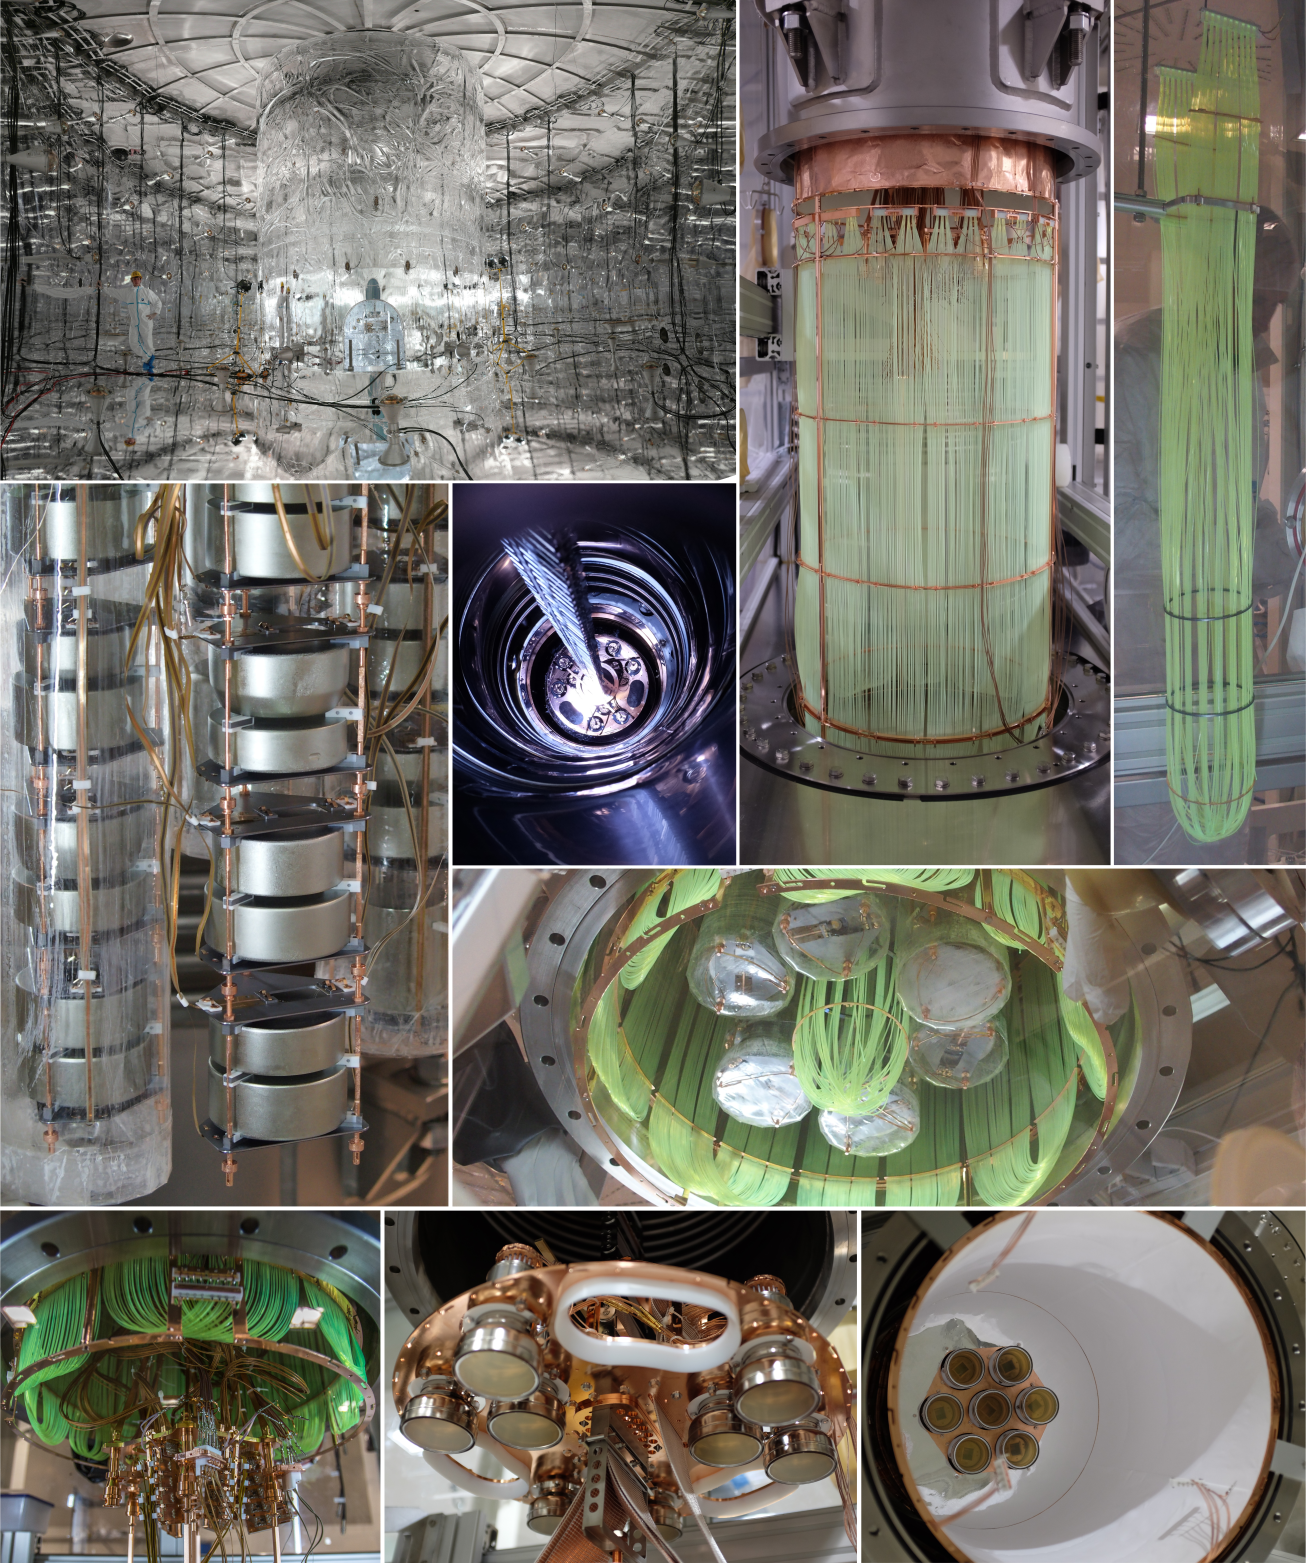
\includegraphics[width=\textwidth]{setup/pic-collage.png}};
    \node[label] at ( 0.3, 17.3) {\emph{a}};
    \node[label] at ( 8.7, 17.2) {\emph{b}};
    \node[label] at (12.8, 17.2) {\emph{c}};
    \node[label] at ( 0.3, 11.8) {\emph{d}};
    \node[label] at ( 5.4, 11.9) {\emph{e}};
    \node[label] at ( 5.4,  7.5) {\emph{f}};
    \node[label] at ( 0.3,  3.6) {\emph{g}};
    \node[label] at ( 4.7,  3.6) {\emph{h}};
    \node[label] at (10.0,  3.6) {\emph{i}};
  \end{tikzpicture}
  \caption{%
    Various pictures of the \gerda\ \phasetwo\ setup, taken during the upgrade works.
    \emph{a)} the muon veto instrumentation inside the water tank; \emph{b)} the light
    guiding outer fiber shroud; \emph{c)} the central fiber shroud; \emph{d)} \phasetwo\
    array closeup, \bege\ detector strings with their holder mounting and WLS mini-shroud
    are visible; \emph{e)} the array being lowered into LAr; \emph{f)} the end cap of the
    central fiber shroud is visible from below the assembled array; \emph{g)} the
    electronics front-end; \emph{h)} the top PMTs and holes for calibration sources;
    \emph{i)} the bottom PMTs in the Tetratex\reg-coated copper shroud.
  }\label{fig:setup:pictures}
\end{figure}

\blocktitle{calibration \\ system}
The \gerda\ weekly calibrations are performed by lowering three \Th\ sources into LAr in
the close vicinity of the array, at the same radial distance from the array central axis
and evenly spaced. Each source, when lowered, just fits into the space between the
cylinder of the LAr veto system and two neighboring outer strings of the detector array,
thereby the sources enter the inner volume of the LAr veto system by three slots in the
top PMT plate.  Three sources were produced and characterized for the first part of
\phasetwo~\cite{Baudis2015} and then again for \phasetwop. The LAr veto instrumentation is
usually switched off during calibration runs because of the too high source activity of
$\mathcal{O}(10)$~kBq.  However, less intense \Ra\ sources are also available and can be
easily exchanged with the standard ones. Special calibration data has been acquired with
these sources and the LAr light instrumentation turned on, to study the performance of the
LAr veto system. The calibration of the experimental setup is extensively described
in~\cite{calib-paper}.

\blocktitle{data \\ acquisition}
A FADC system records traces from germanium detectors (40), PMTs (16) and SiPMs (15) of
the LAr veto, PMTs and scintillating panels of the muon veto when an energy deposition
greater than about 100~keV occurs in at least one of the germanium detectors\footnote{The
  exact trigger threshold is detector- and run-dependent and varies between 20~keV and
200~keV.}. Besides of real physical triggers, two special artificial events are recorded
by the DAQ: test signals injected with a pulser in each germanium detector and baseline
events with no physical trigger to study the electronic noise. These events are recorded
at fixed time intervals during data taking. Since the outset, \gerda\ has adopted a
rigorous blind analysis strategy to ensure an unbiased search for \onbb\ decays. Events with
a reconstructed energy of $\qbbM \pm 25$~keV are blinded (i.e., removed from
the data stream) until the data selection is fixed.
\newpar
The energy deposition associated to each germanium detector signal is
determined via a Zero Area Cusp (ZAC) filter which is optimized off-line for each detector
and each calibration run~\cite{Agostini2015}. PMT and SiPM hits are reconstructed in the
offline analysis following the procedure documented in~\cite{Agostini2018a}. Each event
has to pass a series of quality cuts tailored to discard unphysical events with very high
efficiency (see \cref{sec:gerda:cuts}). The reconstructed trigger positions are converted
into time differences relative to the first trigger found in the germanium detector
traces. Trigger positions and amplitudes are subsequently used together with hits from the
SiPMs and PMTs to test the LAr veto condition. The algorithms were implemented in the \gelatio\
framework~\cite{Agostini2011} which is used to process \gerda\ data. Each event is
characterized by the calibrated energy deposited in the Ge diode, a data quality flag, the
classification as signal or background event from the pulse shape analysis, and veto flags
from the muon veto and LAr veto systems.

\begin{figure}
  \centering
  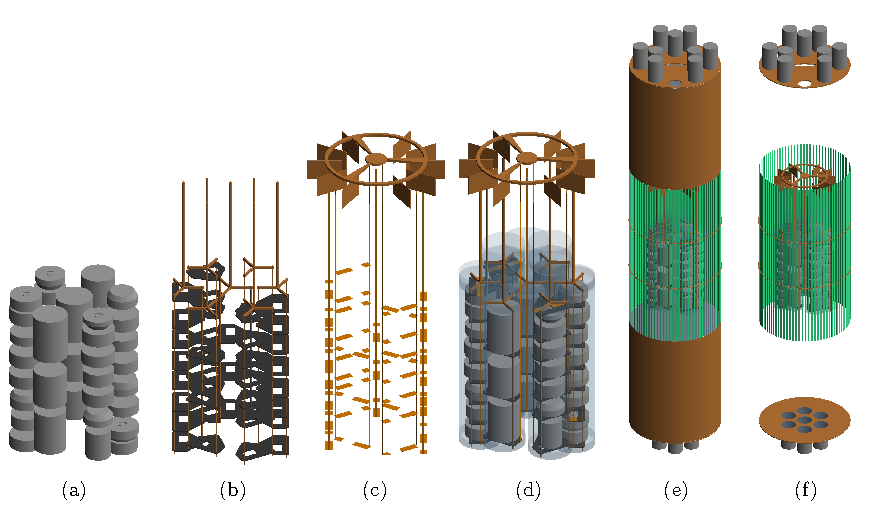
\includegraphics[width=\textwidth]{setup/mage-volumes.pdf}
  \caption{%
    Implementation of the \gerda\ array in \mage, displayed using the \geant\
    visualization drivers. From left to right: \emph{a)} the \phasetwo\ holder mounting,
    composed of silicon plates and copper bars, and the high-voltage and signal flex flat
    cables.  Front-end electronics are on the top end, \emph{b)} the full \phasetwo\ array
    instrumentation, including the transparent nylon mini-shrouds, \emph{c)} the full
    \phasetwop\ array instrumentation, including the central fiber shroud (in green),
    \emph{d)} the full \phasetwo\ LAr veto system, including the outer fiber shroud, the
    Tetratex\reg-coated copper shrouds (above and below the fibers) and the two PMT
    arrays, \emph{e)} the \phasetwop\ LAr veto system without the copper shrouds.
  }\label{fig:setup:magevolumes}
\end{figure}

\section{Background reduction techniques}%
\label{sec:gerda:cuts}

\begin{figure}
  \centering
  \includegraphics[width=\textwidth]{gedet/gerda-events.png}
  \caption{%
    Signal and background events in \gerda, working principles of the main background
    reduction techniques. From left to right: \emph{signal-like events}: the point-like
    topology in dense detectors of double-beta decays generate distinct single-detector
    pulse shapes. \emph{granularity cut}: external, background \g{}s can deposit energy
    in multiple detectors. \emph{pulse-shape discrimination}: insights on the event
    topology can be obtained by analyzing its waveform. Single-site events, multi-site
    events, \b{}s and \a{}s on the surface can be discriminated with offline algorithms
    depending on the specific detector geometry. \emph{LAr veto}: background events that
    deposit energy in germanium and LAr at the same time can be efficiently vetoed by
    the \gerda\ LAr veto. Drawings have been
    created through the \m{gedet-plots} library\textsuperscript{\ref{footnote:gedetplots}}.
  }\label{fig:gerda:event-types}
\end{figure}

Various background mitigation techniques are adopted, both at the data acquisition level
(online) and the analysis level (offline) in \gerda\ to lower the background index to the
background-free level of \pIIbi. The techniques outlined in the following have been
gradually developed and refined during several years of research and publications, and
have been employed for the \phasetwo\ final (re-)analysis in~\cite{Agostini2021}.
Documentation about partial analyses of the \gerda\ \phasetwo\ data published
in~\cite{Agostini2015a, Agostini2017, Agostini2018, Agostini2019a} can be found in those
publications and references therein.

\blocktitle{muon veto}
Muons may cause a substantial background to rare event searches like \gerda\ by generating
counts at \qbb\ either through direct energy deposition in the detectors or through
e.g.~decay radiation of spallation products. At LNGS the cosmic muon flux is reduced by a
factor of ${\sim}10^6$ to a rate of ${\sim}3.4 \cdot 10^{−4}~\text{s}^{-1}\text{m}^{-2}$,
which is sill sufficient to generate a non-negligible background of the order of
\powctsper{-3}.  As already described in \cref{sec:gerda:setup}, a muon veto comprising of
a water \v{C}erenkov veto and a scintillator veto was implemented in \gerda\ to reduce
this background contribution. An event with energy deposition in germanium is flagged
as muon-induced background if a coincidence with the muon veto signal occurs in a $\pm
10$~\mus\ window around the germanium trigger. The efficiency of the muon veto system
has been estimated to be of ${\sim}99$\%, leading to a residual background index of
${\sim}$\powctsper{-5}~\cite{Freund2016}.

\blocktitle{LAr veto}
The primary role of liquid argon in \gerda\ is to keep the germanium detectors at a
cryogenic operational temperature and provide a passive shielding medium against external
backgrounds. Moreover, the LAr can be also employed as a detector medium in an active veto
system, thanks to its scintillation properties. The production mechanism of the
scintillation light in LAr is known since several decades and is deeply described in
literature and its spectrum is today well known. The incident particles deposit their
energy mainly by interactions with the electron shell of the argon atoms which leads to
either an excitation or an ionization of argon atoms. Excited argon atoms are frequently
called `excited dimers' or `excimers' in the literature. Their decay is accompanied by the
emission of scintillation light in the vacuum ultraviolet region, whose typical wavelength
is usually cited as $\lambda = 128$~nm~\cite{Heindl2010}. The ratio between excitation and
ionization is strongly dependent on the pressure and density of the argon as well as on
the type of radiation itself. In the case of excitation, the excited argon atom can
directly form an excimer via the collision with neighboring argon atoms. The process is
sketched in \cref{fig:setup:lar-scint}.
\begin{figure}
  \centering
  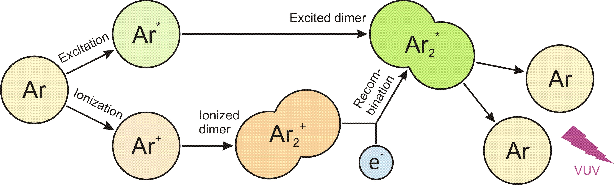
\includegraphics[width=0.7\linewidth]{lar-scint-mechanism.pdf}
  \caption{%
    Scintillation mechanism of liquid argon (or gaseous argon) via the decay of excited
    dimers. The excited dimer can be either formed directly from an excited argon atom or
    from an ionized atom which forms an ionized dimer before its recombination and the
    following recombination in its molecular form. Drawing courtesy of Christoph
    Wiesinger.
  }\label{fig:setup:lar-scint}
\end{figure}
The excimer itself is meta-stable and appears in two different states: the singlet and the
triplet state~\cite{Jortner1965, McCusker1984}.  The decay of the triplet state is
forbidden due to angular momentum conservation, while the decay of the singlet state is
allowed. Consequently the lifetime of the triplet state is 1.59~\mus\ which is
significantly higher than the 6~ns of the singlet state. The scintillation light yield
(combined for both components) is roughly 40 photons/keV, measured in ultra-pure
LAr~\cite{Doke1988}. This value is dependent on different factors, like the presence of
contaminants, the pressure and density of the argon as well as the ionization density of
the incident particle~\cite{Doke1988}.
\newpar
The goal of the \gerda\ LAr veto is to reject those types of background events in the
germanium detectors that simultaneously deposit energy in the surrounding LAr, and hence
generate scintillation. These background types mainly include \g-ray background from Ra
and Th decays in solid materials inside and around the detectors. But also other types of
background can successfully be rejected, such as muons or decays from \Arh\ or \kvz. An
event depositing energy in the germanium detectors is discarded as background if a
coincidence with the LAr veto signal is found in the time window spanned by the germanium
traces.  Since the lifetime of the LAr triplet state significantly depends on the argon
purity~\cite{Amsler2007}, it is possible to monitor the purity of LAr over time.
\cref{fig:lar:triplet-lifetime} shows the lifetime values measured about every month since
the start of \phasetwo. The average measured lifetime dropped after the \phasetwop\
upgrade works from $\sim$1~\mus\ to $\sim$0.9~\mus, as a probable consequence of
maintenance works of the cryogenic system.
\begin{figure}
  \centering
  \includegraphics{plots/lar/lar-triplet.pdf}
  \caption{%
    LAr triplet lifetime regularly measured during \phasetwo. The decrease of the LAr
    purity in 2018 might be attributed to maintenance works of the cryogenic
    infrastructure.
  }\label{fig:lar:triplet-lifetime}
\end{figure}
The veto condition is realized when the signal in at least one channel (SiPM array or PMT)
exceeds a certain threshold (around one photo-electron or less) within a certain time
window around the germanium trigger (usually few microseconds). The \onbb-signal
efficiency of the LAr veto cut can be estimated by evaluating the number of test pulses
and baseline events that are randomly flagged as background events. This fraction has been
evaluated to $(97.7 \pm 0.1)$\% and $(98.2 \pm 0.1)$\% for the first part of \phasetwo\
and \phasetwop, respectively. Combining these two estimates for the whole \phasetwo\
results in an efficiency for \onbb\ events of
\[
  \epsilon_\onbbM^\text{LAr-veto} = (97.92 \pm 0.07)\% \;.
\]

\blocktitle{granularity \\ cut}
Since the topology of \onbb-decay events in germanium is, to a good approximation,
point-like, all events in which energy is simultaneously deposited in more than one
detector can be classified as background. In the offline analysis of a physical event, a
trigger algorithm is applied over all the germanium traces to determine the presence of
other signals besides the main trigger. This `offline' trigger threshold can be as low as
the electronic noise and accounts for possible electronic crosstalk effects between
channels. \fillme{mention AC detectors}

\blocktitle{data \\ quality}
Each event has to pass a series of quality cuts tailored to discard unphysical events such
as discharges, pile-up, overflowed events and other problematic traces with very high
efficiency. The \onbb-signal efficiency of the data quality cuts has been estimated by
building an artificial signal-like data sample and applying the data quality cuts to it.
The base for this data sample consists of special pure-baseline events without physical
triggers, which are regularly recorded in \gerda. Since these events are artificially
triggered, no signal is expected in any detector with high probability, and therefore they
can be used to characterize the background noise at a given time during data taking. On
top of these baseline events special averaged waveforms from \Th\ DEP events are added to
baseline events (only one channel per event) to produce the signal-like sample. An
estimation of the acceptance of these events is finally yields:
\[
  \epsilon_\onbbM^\text{QC} = (99.922 \pm 0.002)\% \;.
\]

\blocktitle{pulse-shape \\ discrimination}
The drift of charges created by a ionizing particle in a voltage-biased germanium
detector, which determines the shape of recorded event waveform, depends on the electric
field in the diode. The latter, in particular, depends on the geometry and on crystal
parameters like the impurity concentration and its gradient. Therefore, analysis
techniques can be developed to discriminate between various event types in germanium
detectors. Distinguishing between single-site (SSE) and multi-site (MSE) events is of
primary interest for \gerda, since \onbb\ decays pertain to the SSE class. The two
electrons, in fact, deposit their energy in germanium within 1~mm$^3$ and can be therefore
considered as point-like events. On the other hand, background events caused by
e.g.~multiple Compton scattering of external \g\ rays are mostly of the multi-site type.
Besides MSEs, surface events are another prominent source of background. Energetic \b\
rays created at the \nplus\ electrode surface can penetrate the dead-layer and deposit
energy in the active volume. In particular, the \b\ decay of \kvz, a daughter of \Arh\
naturally present in LAr, is a dangerous background in the ROI because of its high
Q-value. These \b\ decays at the \nplus\ surface can create `slow' pulses with incomplete
charge collection because of the low electric field in the Li-diffused region. The \pplus\
electrode and the insulating groove can be trespassed also by \a\ particles. The
shallowness of the boron implantation of the \pplus\ (hundreds of nanometers) and the
absence of any dead layer in the groove\footnote{The passivation layer, if present, is
usually hundreds of nanometers thick and can be therefore penetrated by \a\ particles.}
let external \b{}s and \a{}s deposit energy in the detector active volume. The intense
electric field causes energy depositions in this region to generate pulses with short
rise times. \a\ events on the \pplus\ electrode are mainly produced by \Po\ accumulated
on its surface, most probably during detector handling. These 5.3~MeV \a\ particles may
lose part of their energy before reaching the active volume and contribute to the
background in the ROI.
\newpar
To mitigate all these background sources, pulse-shape discrimination (PSD) techniques were
developed separately for \bege, \icoax\ and \scoax\ detectors separately, to be applied
after the LAr veto cut. For the first class a simple univariate cut was sufficient, while
for the latter two techniques were worked out, one based on neural networks and one on the
analysis of the rise time of the pulses.  In order to avoid systematic effects
calibration, training and evaluation of the PSD methods should be performed on pulses with
energies close to these of the expected signal at \qbb.  In practice, appropriate event
sets are extracted from the weekly \Th\ calibration spectra. The PSD methods applied to
the \gerda\ data are briefly outlined in the following. The interested reader is referred
to~\cite{Agostini2021a} for a detailed treatment of the topic. \fillme{define somewhere FEP,
SEP and DEP}

\blocktitle{PSD for \\ \bege{}s and \\ \icoax{}s}
PSD for point-contact detectors (\bege\ and \icoax) is based on the \aoe\ ratio, where $A$
is the maximum amplitude of the current signal and $E$ is the event energy. This technique
has been extensively studied in the past in the context of \gerda~\cite{Agostini2013,
Agostini2010, Budjas2008, Budjas2009, Budjas2009a, Agostini2010a}. The motivation in
employing such a relatively simple, univariate cut lies in the observation that in
\bege\ and \icoax\ detectors, thanks to their small \pplus\ contact, the electric field
has a special distribution, resulting in the same shape of pulses induced by drifting
holes along paths near the \pplus\ electrode~\cite{Agostini2010}. Multiple energy
depositions in the detector can be treated as a superposition of several single
interactions. It follows that a MSE will have a lower $A$ compared to a SSE with the
same $E$.  A two-sided cut on \aoe\ to cut MSEs slow pulses and \pplus\ fast events is
introduced and determined separately for each detector. Energy and time stability
corrections to \aoe\ are discussed in detail in~\cite{Agostini2021a}. As mentioned before,
the \aoe\ cut values are determined employing representative data samples from \Th\
calibration runs.  The low cut position (rejection of MSEs and slow pulses) is adjusted
to achieve a 90\% survival fraction of the double-escape peak (DEP), a SSE sample. The
threshold on the high \aoe\ side (rejection of fast pulses) has been fixed to 3 standard
deviations away from the SSE band distribution. The survival fraction for the
\onbb-decay signal has been calculated assuming that it is the same as for the DEP
events. A full analysis of the statistical and systematic uncertainties yields
\[
  \epsilon_\onbbM^{A/E} = (88.7 \pm 2.3)\% \;.
\]
for the combined \bege\ and \icoax\ data sets.

\blocktitle{PSD for \\ \scoax{}s}
In semi-coaxial detectors the length of the drift path of the holes depends on the
location of the energy deposition and it induces different types of pulse shapes. Because
of this reason, a simple \aoe\ cut would not be as effective as for the \bege{}s, and
therefore alternative methods have been worked out.
\newpar
The primary method to reject MSE, called here \annmse, consists in a TMVA-based artificial
neural network\footnote{\url{https://root.cern/tmva}} and requires appropriate selection
of input variables (from the rising part of the preamplifier charge pulse) and training on
independent data samples. Several of these samples are available for training in
calibration data (see \cref{fig:gerda:calib-desc}, top) and also in physics data (\kvz\
full-energy peak, \nnbb\ events, \a-induced events). The \annmse\ is specifically trained
on \Th\ calibration data, selecting the \Tl\ DEP as a SSE sample and the \Bil\ FEP at
1621~keV as a MSE sample. The classifier cut threshold is then fixed to a 90\% survival
probability for the \Th\ DEP, and the cut signal efficiency is calculated from Monte Carlo
simulations of \onbb-decay events. The obtained \annmse\ signal survival fraction is
$(82.2 \pm 3.7)$\%.
\newpar
\a-induced events on the \pplus\ electrode surface are rejected by a separate method based
on the analysis of the pulses rise time (RT). These events are generally characterized by
a fast collection time, and their charge collection might be delayed or partial, if
originated in the proximity of the groove. The RT cut exploits the fast rise time of these
\a\ events and is therefore equivalent to a volume cut, which excludes the surfaces
vulnerable to the \a-induced events. The rise time is defined as the time the waveform
needs to reach from 10\% to 90\% of its amplitude. The RT-cut threshold is defined to
maximize the \onbb\ survival fraction and to minimize the signal-to-noise ratio at the
same time through the definition of a figure of merit defined as the product of the \nnbb\
signal survival square-probability and the \a-events rejection probability. The \nnbb\ and
\a-event test samples are obtained from physics data by selecting data in the $[1.0,
1.3]$~MeV and $>3.5$~MeV energy regions, respectively, after \annmse\ and LAr veto cuts.
The \onbb-signal efficiency of the RT cut is assumed to be the same as for the \nnbb\
decays and hence estimated to 82.3\%, with an uncertainty of the order of
1\%~\cite{Lazzaro2019}.

\blocktitle{\deltae\ cut}
Events featuring slow charge collection might suffer from ballistic deficit in the ZAC
energy reconstruction~\cite{Agostini2015} and survive the PSD cuts, especially in
semi-coaxial detectors. Therefore an additional rejection criteria is applied based on the
energy reconstructed with different integration times. The figure of merit for such a cut
is the ratio between the energy of an event reconstructed with a short (4~\mus)
integration time $E_\text{s}$ and the energy reconstructed with a long (20~\mus)
integration time $E_\text{l}$. The energy here is reconstructed using a gaussian-shaping
filter, which has been the default \gerda\ energy reconstruction method for \phaseone.
Ballistic deficit is observed to reduce this ratio, therefore the \deltae\ classifier is
defined as $\delta{E} = E\cdot({[E_\text{s}/E_\text{l}]}_\text{norm} - 1)$, where the energy ratio
is normalized to the values assumed by the \Th\ FEP events. The normalization is applied
in a certain calibration validity period and for each detector separately. The cut value
is defined as 3 negative standard deviations away from the mean of the FEP \deltae\
distribution. The survival fraction of \nnbb\ events, which provides an estimate of the
\onbb\ efficiency, is higher than 98\% for all detector types. It has been estimated,
after all the other PSD cuts, to $(99.449 \pm 0.006)$\% for \scoax, $(99.9572 ± 0.0003)$\%
for \bege\ and 100\% for \icoax\ detectors separately.  A weighted combination yields:
\[
  \epsilon_\onbbM^\text{\deltae} = (99.769 \pm 0.002)\% \;.
\]

The \annmse, RT, \aoe\ and \deltae\ cut efficiencies can be combined to obtain an overall
survival fraction for the \onbb-decay events after the PSD cut:
\begin{center}
  \begin{tabular}{cc}
    \mc{2}{Before upgrade (\%)}     \\
    \midrule
    \scoax\        & \bege\         \\
    $69.1 \pm 5.6$ & $88.2 \pm 3.4$ \\
  \end{tabular}
  \hspace{0.5cm}
  \begin{tabular}{ccc}
    \mc{3}{After upgrade (\%)}                       \\
    \midrule
    \scoax\        & \bege\         & \icoax\        \\
    $68.8 \pm 4.1$ & $89.0 \pm 4.1$ & $90.0 \pm 1.8$ \\
  \end{tabular}
\end{center}
Combining all data together one gets
\[
  \epsilon_\onbbM^\text{PSD} = (80.8 \pm 2.1)\%
\]
as total \onbb\ PSD signal efficiency for the \phasetwo\ data set.

\section{Final \gerda\ data analysis}%
\label{sec:gerda:ana}

The \phasetwo\ single-detector data is presented in this section together with the LAr
veto and PSD data.  The statistical analysis used to extract a lower limit for the \onbb\
half-life in \gesix\ is finally presented, and the final results for the combined \gerda\
data are given.

\begin{figure}
  \centering
  \includegraphics{plots/0nbb-results/calib/supercalib.pdf}
  \caption{%
    Top panel: \Th\ calibration summed spectra of \bege, semi-coaxial and inverted-coaxial
    detectors as used to determine the energy resolution curves. Bayesian blocks are used
    to display the histograms (see \cref{apdx:bayesblocks}). Three prominent \Tl\ high
    energy peaks (full-energy, single-escape and double-escape) and the \Bil\
    single-escape peak at 1621~keV are highlighted. Bottom panel: extracted peak widths
    (FWHM) and fitted calibration curves for pre- and post-upgrade data separately. Points
    represented by empty markers are excluded from the fit because of additional effects
    that contribute to the width. Triangles label peaks broadened by the Doppler effect
    \fillme{ref?}, diamonds label summation peaks.
  }\label{fig:gerda:calib-desc}
\end{figure}

\blocktitle{energy \\ scale and \\ resolution}
As already emphasized in \cref{sec:nbb:exp}, a good energy resolution is a key ingredient
to achieve a high \onbb-decay sensitivity. The main goal of the calibration analysis is
therefore to define and maintain a stable energy scale over years of data taking.  It
is necessary to identify the peak region (and reject all background events with
different energy), combine data from different detectors over extended periods of time,
and efficiently exploit the excellent energy resolution of germanium detectors.
\newpar
As already mentioned in \cref{sec:gerda:setup}, the germanium detectors are calibrated by
exposing them to \Th\ sources with an activity of about 10~kBq. A typical calibration
spectrum is shown in \cref{fig:gerda:calib-desc}. The pattern of \g\ lines in the spectrum
can be exploited to identify certain \g\ lines and calibrate the energy scale of a
detector with their known position in terms of energy. Additionally, the resolution of a
detector can be determined from the width of the \g\ lines. Once the positions and the
widths of the \g\ lines in an energy spectrum is determined by modeling the peaks with a
suitable analytical function, an function interpolation is performed to obtain the energy
calibration and resolution at other energies. Once these two curves are determined for a
given calibration, they are assumed to be valid until the next one. This validity is
constantly monitored by evaluating the shift of the pulser event energy over time with
respect to its value right after a calibration. Time periods in which in which a detector
shows deviations from its calibration above a certain threshold are removed from the final
analysis in order to meet the stringent requirements for the \onbb\ analysis in terms of
uncertainties on the energy scale and resolution. Fluctuations below this threshold are
taken into account when estimating the systematic contribution to the uncertainty on the
energy resolution. The stability of the energy scale and resolution is also monitored on a
per-calibration basis, and time periods for which detectors show a degraded performance
are excluded from combined analysis data sets.  The calibration spectra that refer to
these combined data sets are obtained by summing together the spectra from all the
calibration runs of the relative time period weighted by their actual validity in time.
Gaussian mixtures are usually not needed to model peaks in these combined spectra, as the
variance of the single centroids and widths is usually small enough to enable the use of
single gaussian distributions with effective parameters. The effective data set energy
resolution is then determined by fitting the square root of a linear function to the
reconstructed \g-line widths. The uncertainty on this effective resolution includes
systematic contributions from the choice of the peak model, the resolution function and
time stability of the experimental setup.  The resolution curves for \bege, semi-coaxial
and inverted-coaxial \phasetwop\ data sets are reported in \cref{fig:gerda:calib-desc} as
an example. The energy resolution at \qbb\ (FWHM) for \phasetwo\ is the following:
\begin{center}
  \begin{tabular}{cc}
    \mc{2}{Before upgrade (keV)}  \\
    \midrule
    \scoax\       & \bege\        \\
    $3.6 \pm 0.3$ & $2.9 \pm 0.3$ \\
  \end{tabular}
  \hspace{0.5cm}
  \begin{tabular}{ccc}
    \mc{3}{After upgrade (keV)}                   \\
    \midrule
    \scoax\       & \bege\        & \icoax\       \\
    $5.2 \pm 1.9$ & $2.6 \pm 0.2$ & $2.9 \pm 0.1$ \\
  \end{tabular}
\end{center}
The calibrated energy spectrum of the \gerda\ \phasetwo\ data after granularity cut is
shown in \cref{fig:gerda:physics-spectra}, empty histogram.

\begin{figure}
  \centering
  \includegraphics{plots/0nbb-results/physics-spectra.pdf}
  \caption{%
    Single-detector data from the enriched detectors is displayed in a combined spectrum
    after indicated cuts. Main contributions to the spectra are labeled in the top panel.
    The bottom-left panel shows data in the \qbb\ region. Known \g\ peaks and the \onbb\
    analysis window are highlighted in gray and green, respectively. The bottom-right
    panel shows the unbinned data after all cuts in the analysis window and the fit
    results.
  }\label{fig:gerda:physics-spectra}
\end{figure}

\blocktitle{LAr veto and \\ PSD cuts on \\ data}
The first cut applied to \phasetwo\ data (after the quality cuts and the multiplicity cut)
is the LAr veto cut.  Event energy histograms before and after this event selection are
shown in \cref{fig:gerda:physics-spectra}. The cut clearly suppresses background events from
the \Th\ and \Uh\ decay chains, as well as \kvz\ events. The \kvz\ FEP event reduction to
20\% and 18\% in \phasetwo\ and \phasetwop\ data, respectively, demonstrates the
effectiveness of the improved fiber instrumentation installed for \phasetwop. \kvn\
events, which are characterized by a single \g\ emission at 1461~keV and typically do not
deposit energy in LAr, show a high survival fraction of about 98\%, but cannot enter the
ROI at 2039~keV and are therefore of minor concern. \a\ events that dominate the energy
spectrum at higher energies cannot be vetoed but the LAr instrumentation and still
constitute a major background at \qbb.
\newpar
PSD data versus energy is showed in \cref{fig:gerda:psd-on-data} subdivided according to
the PSD method. Data from \bege\ and inverted-coaxial detectors, for which the \aoe\ cut
is used, is shown in the top-left plot. Data from semi-coaxial detectors, for which the
\annmse\ and the rise-time cuts are implemented, is shown in the remaining plots. Colored
data points correspond to events that survive the PSD cut.

\begin{figure}
  \centering
  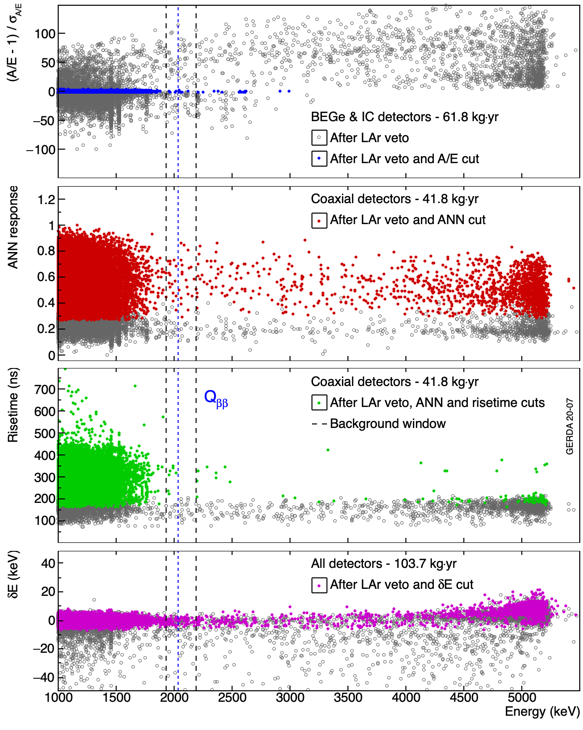
\includegraphics[width=0.9\textwidth]{plots/0nbb-results/G2006_all_psd0.png}%
  \caption{%
    The four pulse shape discrimination techniques applied on the final \gerda\ \phasetwo\
    data set. From top t0 bottom: the \aoe\ cut, the \annmse\ cut, the
    rise-time cut and the \deltae\ cut. Note that, being the \deltae\ cut
    highly-correlated with \aoe\ in \bege\ and \icoax\ detectors, its direct application
    on data after the LAr veto cut results in a high cut efficiency. If applied after all
    others PSD cuts, the event survival fraction is >99\%.
  }\label{fig:gerda:psd-on-data}
\end{figure}

The energy range considered for the \onbb\ statistical analysis goes from 1930~keV to
2190~keV, excluding the two regions $2014 \pm 5$~keV and $2119 \pm 5$~keV in which two
known \g\ lines from \Bih\ and \Tl\ lie. No other non-flat background structure is
expected from the background studies that will be presented in the following chapters.
The analysis window is shown in \cref{fig:gerda:physics-spectra}: in green in the bottom
left panel and in the bottom right panel. After the unblinding, 13 events are found in
this analysis window after all cuts (5 in \scoax, 7 in \bege\ and 1 in \icoax detectors).
These avents are likely due to \a\ decays, \kvz\ \b\ decays or \g\ decays from \Uh\ and
\Thh\ series. Data which were unblinded in~\cite{Agostini2017}, when less effective PSD
techniques against surface events were available, have been re-analyzed according to the
new methods described in this work: as a consequence, three events (at energies 1967, 2061
and 2064~keV) that were previously included in the analysis window in past data
releases~\cite{Agostini2019a, Agostini2017, Agostini2018} are now discarded.

\begin{sidewaystable}
  \centering
  \caption{%
    Summary of the parameters of interest for \gerdatwo\ for different detector types and
    before/after the upgrade.  The components of the total efficiency $\epsilon$ for
    \onbb\ decays are also reported individually. The efficiency factors due to muon veto
    and quality cuts are above $99.9\%$ and are not shown explicitly.  Energy resolution
    and all \onbb\ decay efficiencies are reported as exposure-weighted average for each
    detector type and their uncertainties are given as standard deviation.
  }\label{tab:gerda:efficiencies}
  \addfontfeatures{Numbers=Tabular}
\begin{tabular}{rccccc}
  \toprule
                                                 & \mc{2}{Dec 2015 -- May 2018}                      & \mc{3}{July 2018 -- Nov 2019}                                   \\
                                                 & \scoax\                     & \bege\              & \scoax\             & \bege\              & \icoax\             \\
  \midrule
  Number of detectors                            & 7                           & 30                  & 6                   & 30                  & 5                   \\
  Total mass                                     & 15.6~kg                     & 20~kg               & 14.6~kg             & 20~kg               & 9.6~kg              \\
  Exposure \expo\                                & 28.6~\kgyr\                 & 31.5~\kgyr\         & 13.2~\kgyr\         & 21.9~\kgyr\         & 8.5~\kgyr\          \\
  Energy resolution at \qbb\ (FWHM)              & $(3.6 \pm 0.2)$~keV         & $(2.9 \pm 0.3)$~keV & $(4.9 \pm 1.4)$~keV & $(2.6 \pm 0.2)$~keV & $(2.9 \pm 0.1)$~keV \\
  \onbb\ decay detection efficiency $\epsilon$:  & $(46.2 \pm 5.2)\%$          & $(60.5 \pm 3.3)\%$  & $(47.2 \pm 5.1)\%$  & $(61.1 \pm 3.9)\%$  & $(66.0 \pm 1.8)\%$  \\
  \midrule
  \emph{Electron Containment}                    & $(91.4 \pm 1.9)\%$          & $(89.7 \pm 0.5)\%$  & $(92.0 \pm 0.3)\%$  & $(89.3 \pm 0.6)\%$  & $(91.8 \pm 0.5)\%$  \\
  \emph{\gesix\ enrichment}                      & $(86.6 \pm 2.1)\%$          & $(88.0 \pm 1.3)\%$  & $(86.8 \pm 2.1)\%$  & $(88.0 \pm 1.3)\%$  & $(87.8 \pm 0.4)\%$  \\
  \emph{Active volume}                           & $(86.1 \pm 5.8)\%$          & $(88.7 \pm 2.2)\%$  & $(87.1 \pm 5.8)\%$  & $(88.7 \pm 2.1)\%$  & $(92.7 \pm 1.2)\%$  \\
  \emph{Liquid Argon veto}                       & \mc{2}{$(97.7 \pm 0.1)\%$}                        & \mc{3}{$(98.2 \pm 0.1)\%$}                                      \\
  \emph{Pulse shape discrimination}              & $(69.1 \pm 5.6)\%$          & $(88.2 \pm 3.4)\%$  & $(68.8 \pm 4.1)\%$  & $(89.0 \pm 4.1)\%$  & $(90.0 \pm 1.8)\%$  \\
  \bottomrule
\end{tabular}

\end{sidewaystable}

\blocktitle{statistical \\ analysis}
The energy distribution of the events in this window is fitted to search for a \onbb-decay
signal. The baseline fit model includes a Gaussian distribution for the signal, centered
at \qbb\ with a width corresponding to the energy resolution, and a uniform distribution
for the background. The free parameters of the fit are the signal strength $S=1/T$ and the
background index $B$. The number of signal events scales with $S$ as
\begin{equation}\label{eq:gerda:mu_s}
  \mu_s = \frac{\mathcal{N}_A \log2}{m_{76}} \cdot \epsilon \cdot \expoM \cdot S \;,
\end{equation}
where $\mathcal{N}_A$ is the Avogadro number, $m_{76}$ is the \gesix\ molar mass, \expo\
is the total exposure scrutinized and $\epsilon$ is the total \onbb\ detection efficiency.
The efficiency $\epsilon$ accounts for the enrichment fraction in \gesix, the active
volume fraction of the germanium detectors, the electron containment efficiency and the
analysis cuts. The latter include the quality cuts, the muon veto cut, the LAr veto cut
and the PSD cut. The efficiency $\epsilon$ is evaluated on the full \phasetwo\ dataset to
be $(47.0 \pm 3.9)$\% for the \scoax\ detectors $(60.7 \pm 2.5)$\% for the \bege\ detectors
and $(66.0 \pm 1.8)$\% for the \icoax\ detectors. The average total efficiency $\epsilon$
and the breakdown in the individual components are listed in \cref{tab:gerda:efficiencies}
The number of background events in the analysis window is given by
\begin{equation}\label{eq:gerda:mu_b}
  \mu_b = B \cdot \Delta{}E \cdot \expoM \;,
\end{equation}
where $\Delta{}E = 240$~keV is the effective width of the window after removing the two
aforementioned \g-line regions.
\newpar
Data from each detector is divided in partitions, i.e.~periods of time in which parameters
such as the resolution and efficiency are stable. The parameters of each of the 408
partitions are indicated by the index $k$. The signal strength $S$ and the background
index $B$ instead are common parameters to all partitions. This construction constitutes a
significant improvement over the previous data releases~\cite{Agostini2019a, Agostini2018,
Agostini2017} as it allows a precise tracing of the performance of each detector at a
given moment. Another difference compared to the previous analyses is that the background
index is now assumed to be the same for all detectors, while independent parameters were
used in the past for each detector type. There is no statistical evidence indeed that the
background is different between the three detector types, or detector position within the
array, or time.
\newpar
The statistical analysis is based on an unbinned extended likelihood function and it is
performed in both frequentist and Bayesian frameworks, following the procedure described
in~\cite{Agostini2017}. The likelihood function is given by the product of likelihoods of
each partition:
\[
  \mathcal{L} = \prod_k \left[
    \frac{{(\mu_s + \mu_b)}^{N_k} e^{-(\mu_s + \mu_b)}}{N_k!} \times
    \frac{1}{\mu_s + \mu_b} \times
    \prod^{N_k}_{i=1} \left(
      \frac{\mu_b}{\Delta{}E} +
      \frac{\mu_s}{\sqrt{2\pi\sigma_k}} e^{-\frac{{(E_i - \qbbM)}^2}{2\sigma_k^2}}
    \right)
  \right] \;,
\]
where $E_i$ is the energy of the $N_k$ events in the $k$-th partition and $\sigma_k =
\text{FWHM}/2.35$ is the energy resolution of the partition. The parameters $\mu_s$ and
$\mu_b$ are calculated from \cref{eq:gerda:mu_s,eq:gerda:mu_b} respectively and are a
function of the efficiency $\epsilon_k$ and the exposure $\expoM_k$ of each partition.
\phaseone\ data sets are included in the analysis as individual partitions with
independent background indices.
\newpar
The frequentist analysis is performed using a two-sided test statistics based on the
profile likelihood, as described in~\cite{Agostini2017}. The probability distributions of
the test statistic have been computed using Monte Carlo techniques, as they are found to
significantly deviate from $\chi^2$ distributions. The analysis of the $N=13$ events of
\phasetwo\ returns no indication for a signal and a lower limit is set to $\thalfzeroM >
1.5 \cdot 10^{26}$~yr at 90\% C.L. \phaseone\ and \phasetwo\ data together give a total
exposure of 127.2~\kgyr. The combined analysis has also a best fit for null signal
strength, and provides a half-life limit of
\[
  \thalfzeroM > 1.8 \cdot 10^{26}~\text{yr at 90\% C.L.}
\]
The limit coincides with the median expectation under the no-signal hypothesis (i.e.~the
sensitivity): $1.8 \cdot 10^{26}$~yr at 90\% C.L. \gerda\ achieved an unprecedentedly low
background in \phasetwo, as derived from the fit, of $B = \measurementM{5.2}{1.6}{1.3}
\cdot 10^{-4}$~\ctsper, and met the design goal to run the entire \phaseone\ data taking
in the background-free regime: the number of background events expected in the signal
region ($\qbbM \pm 2\sigma$) is in fact 0.3.
\newpar
The statistical analysis is carried out also within a Bayesian framework. The
one-dimensional posterior probability density function $P(S|\text{data})$ of the signal
strength is derived by marginalizing over the other free parameters. the calculation is
performed via a Markov chain Monte Carlo (MCMC) numerical integration osing the Bayesian
analysis toolkit BAT~\cite{Caldwell2008}. The prior distribution for $S$ is assumed to be
constant between 0 and $10^{-24}$~yr$^{-1}$, as in the previous \gerda\ releases. The
limit on the half-life is $\thalfzeroM > 1.4 \cdot 10^{26}$~yr (90\% C.I.). Other choices
for the prior are also possible: as instance, equiprobable Majorana neutrino masses
($\text{prior} \propto 1/\sqrt{S}$). The limit derived in this case is significantly
stronger, $\thalfzeroM > 2.3 \cdot 10^{26}$~yr (90\% C.I.), as the prior gives a higher
probability for low values of $S$.
\newpar
Uncertainties on the energy reconstruction, energy resolution, and efficiencies are folded
into the analysis through additional nuisance parameters, each constrained by a Gaussian
probability distribution in the likelihood. Their overall effect on the limit is at the
percent level. Potential systematic uncertainties related to the fit model have been
studied and found to marginally impact the results. In particular, different background
energy distribution were investigated and it was found that in all cases the limit is
stable within a few percent.

\blocktitle{closing}
\gerda\ is the first experiment to have reached a sensitivity to half-life values above
\powtenyr{26}: with this final data release it is the experiment providing the best
sensitivity and the most stringent half-life constraint of the entire field.
\newpar
The \thalfzero\ limit can be converted into an upper limit on the effective Majorana mass
\mbb\ under the assumption that the decay dominated by the exchange of light Majorana
neutrinos. Assuming a standard value of $g_A = 1.27$, the phase space factors and the set
of most recent nuclear matrix elements calculations, a limit of $m_{\upbeta\upbeta} = 80 -
182$~meV is obtained, which is comparable to the most stringent constraints coming from
other isotopes~\cite{Anton2019, Gando2016, Adams2019}. \gerda\ has been a pioneering
experiment in the search for \onbb\ decay.  In about a decade, \gerda\ improved the
sensitivity by one order of magnitude with respect to previous \gesix\ experiments and
proved that a background-free experiment with \gesix\ is feasible. This paves the way for
the next generation experiment that is currently being prepared by the LEGEND
collaboration.

% vim: tw=90
